\begin{frame} \frametitle{\vspace*{0.5cm}Results: A closer look at how circulation is deposited.}
  Circulation,
  \begin{align*}
    \Gamma = \int_{-\infty}^{+\infty}\int_{0.5\lambda}^{1\lambda}\omega\, \diff x \diff y \qquad \qquad
  \end{align*}
  \vspace*{-0.75cm}
  \begin{figure}
    \centering
    \hfill%
    \begin{tikzpicture}%
      \node[anchor=south west,inner sep=0] (image) at (0,0) {%
        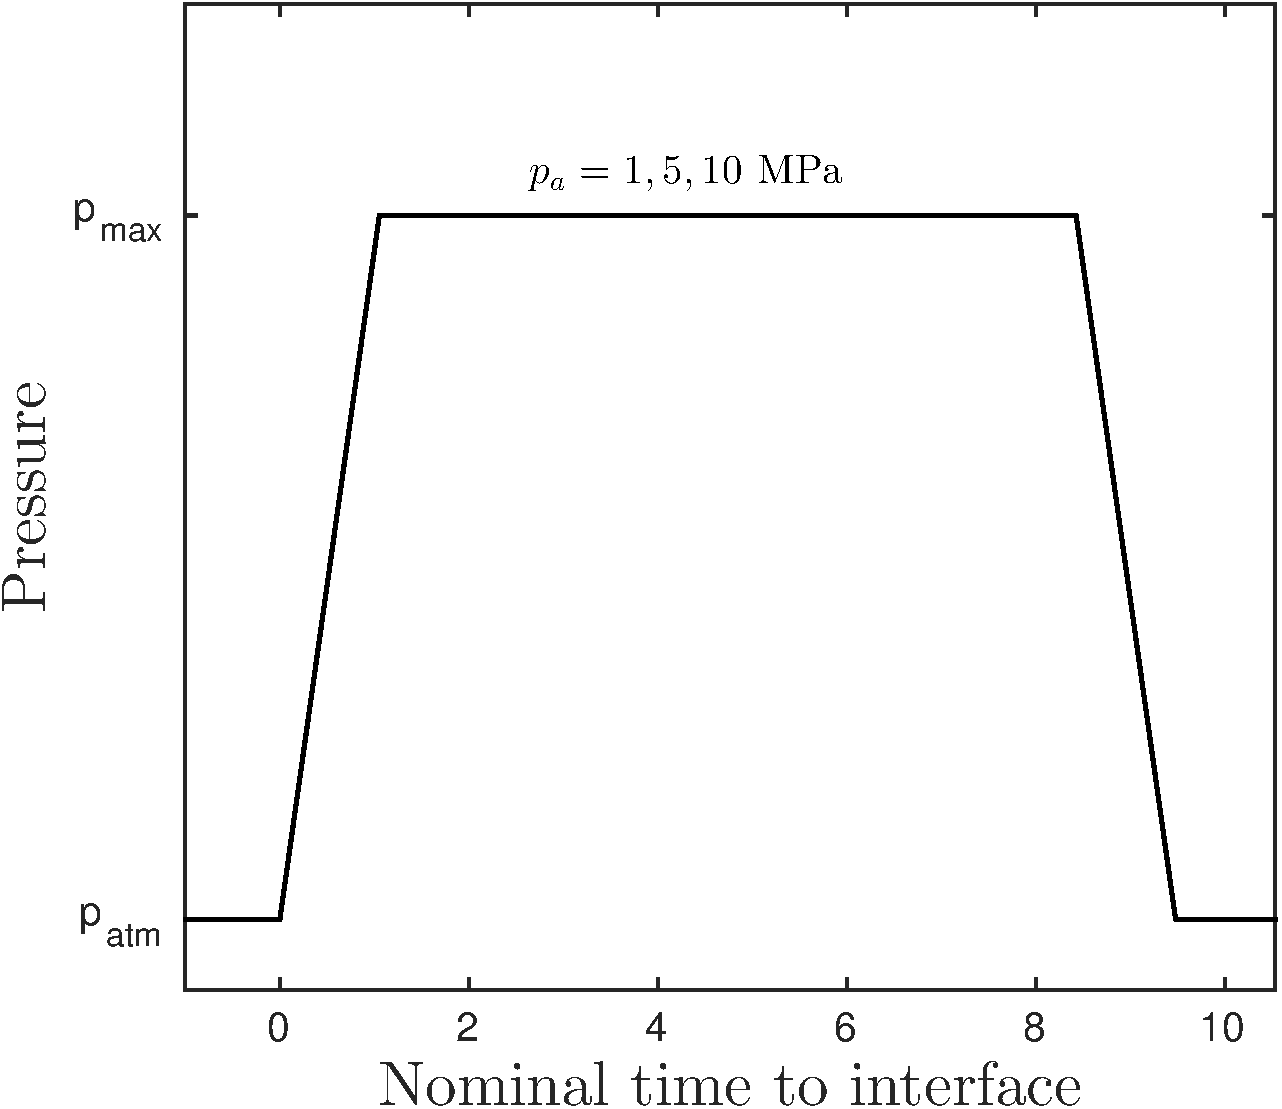
\includegraphics[height=0.43\textheight]{../figs/lung_figs/p0_vs_t_nd.pdf}%
      };%  
      \begin{scope}[x={(image.south east)},y={(image.north west)}]%
        \node[font=\footnotesize,right] at (0.22,0.18){ $t_1$};%
        \node[font=\footnotesize,right] at (0.2,0.8){ $t_2$};%
        \node[font=\footnotesize,right] at (0.83,0.8){ $t_3$};%
        \node[font=\footnotesize,right] at (0.82,0.18){ $t_4$};%
      \end{scope}%  
    \end{tikzpicture}%
    \hfill%
    %
    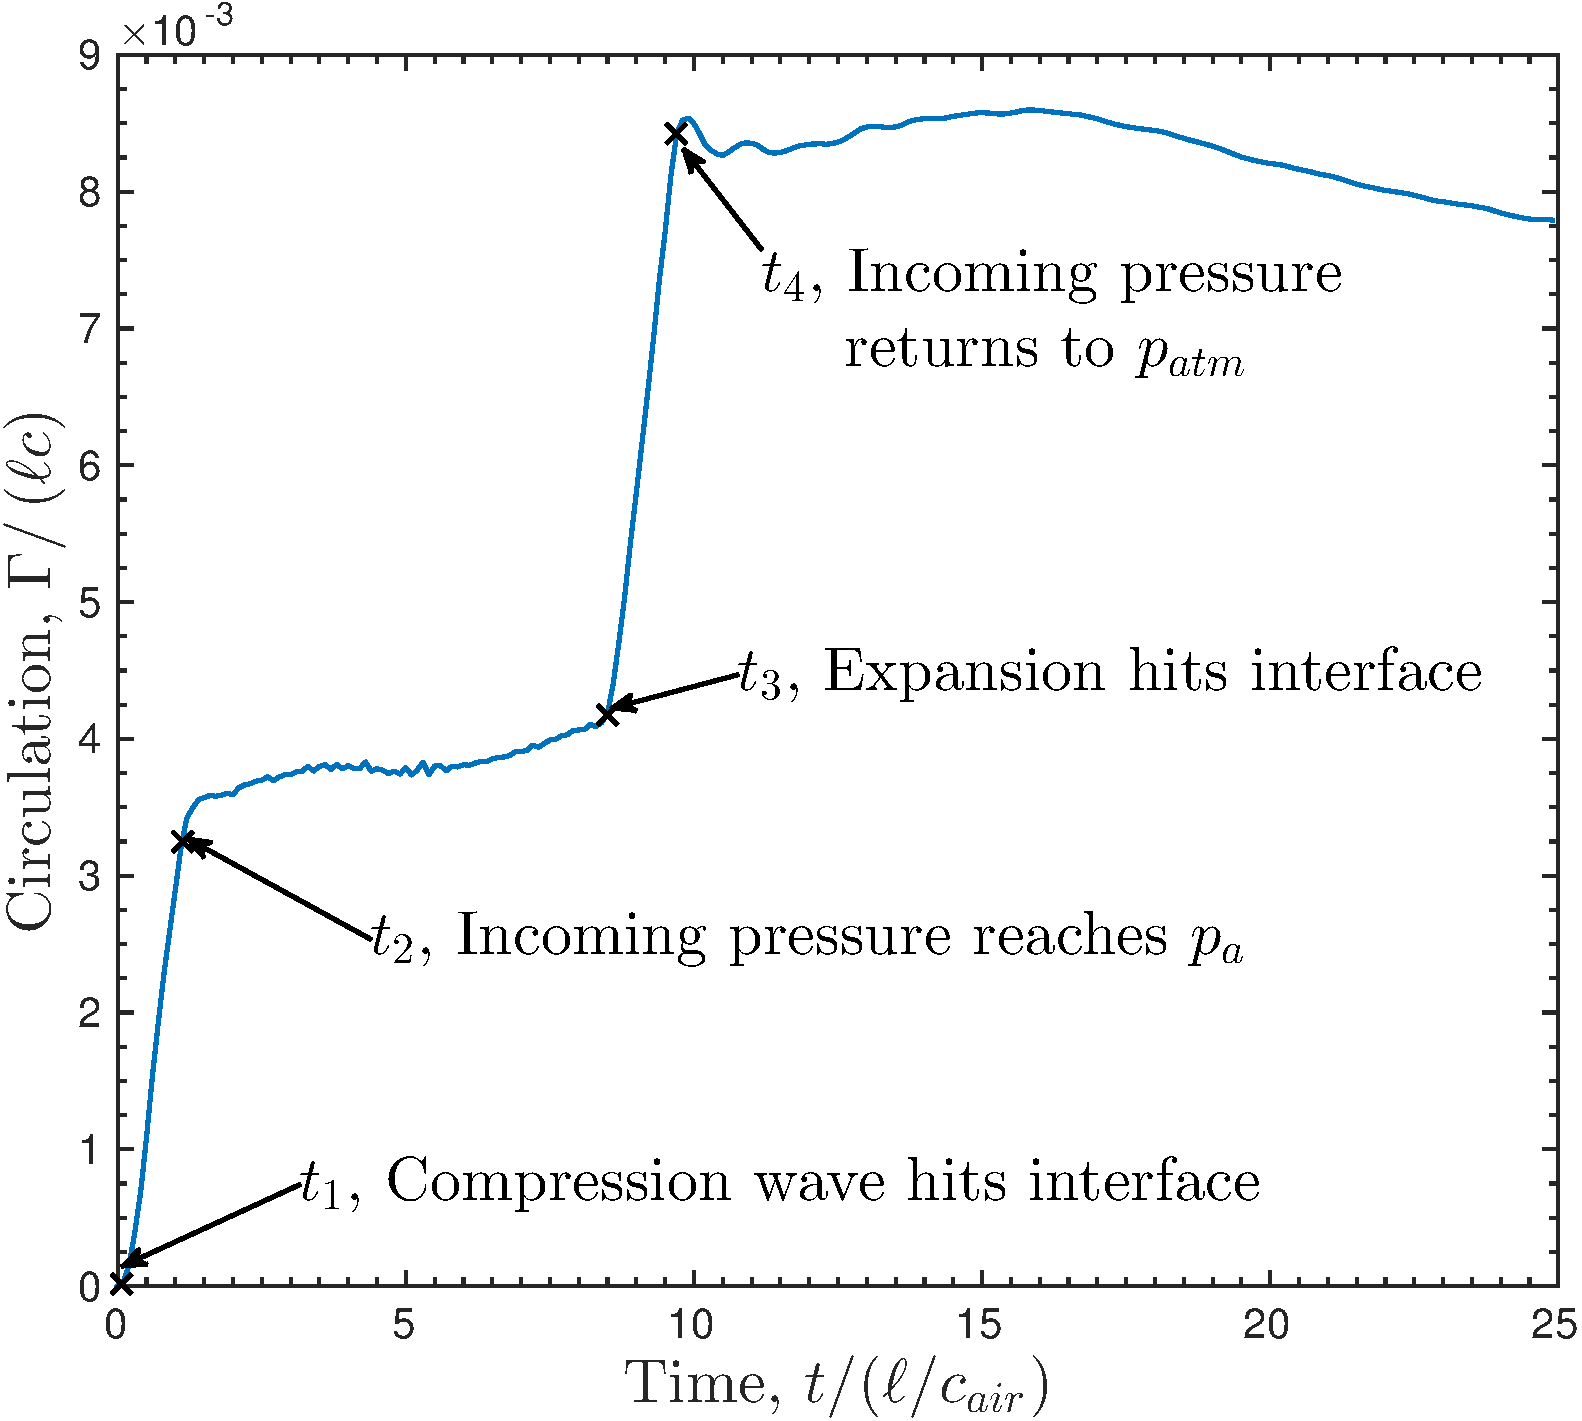
\includegraphics[height=0.43\textheight]{../figs/lung_figs/trapz10_circ_schematic}
    \hfill%
    % 
    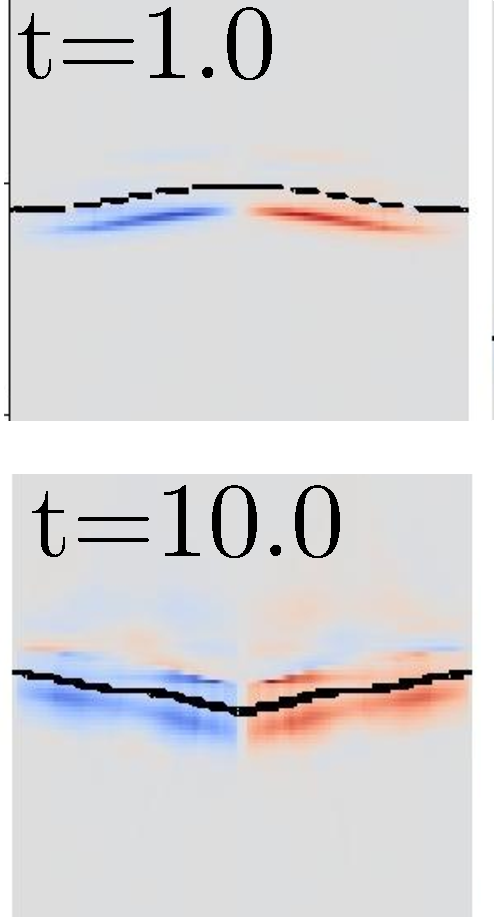
\includegraphics[height=0.43\textheight]{../figs/lung_figs/snapshots_vorticity_t1_t10}%
  \end{figure}
  \begin{itemize}
  \item Both the compression and expansion deposit vorticity.
  \end{itemize}

  \note{ To Do: Label phase-inversion.
    \begin{enumerate}
    \item So to get an idea of the global vorticity, we integrate it
      over the right half domain to get the circulation.
    \item The whole domain circulation is zero because of symmetry.
    \item If we look at the circulation as a function of time relative
      to different parts of the wave interaction, we see that it
      increases for both the compression and expansion.
    \item This is what we expect of baroclinic vorticity, because
      while the pressure gradient has changed sines, the density
      gradient has changed directions as a result of the phase
      inversion.
    \end{enumerate}
    %Mauro's Questions:\\
    %(1) What is the vorticity doing during the phase inversion?
  }
\end{frame}
%%% Local Variables:
%%% mode: latex
%%% TeX-master: "../main"
%%% End:
